\documentclass[a4paper,twoside,kulak]{kulakreport} %options: kul or kulak (default)

\usepackage[utf8]{inputenc}
\usepackage[dutch]{babel}
\usepackage{eurosym}
\usepackage[utf8]{inputenc}
\usepackage[dutch]{babel}
\usepackage{siunitx}
\usepackage{graphicx}
\usepackage{flafter}
\usepackage{pdfpages}
\usepackage{caption}
\usepackage{subcaption}
\usepackage{booktabs}


\faculty{Wetenschap \& Technologie Kulak}
\group{Ingenieurswetenschappen}
\title{How to make \textit{an automated microplate dispenser}}
\subtitle{Een zoektocht naar balans tussen precisie, snelheid en betaalbaarheid}
\author{Team ELISA}
\institute{Matthias Derez, Maxime Dujardin, Korneel Verkens, Seppe Vilain}
\date{Academiejaar 2019 -- 2020}
\address{
   KU Leuven Kulak           \\
   Wetenschap \& Technologie \\
   Etienne Sabbelaan 53, 8500 Kortrijk                \\
   \href{mailto:\theemailaddress}{\texttt{\theemailaddress}}
   }

\begin{document} % hier begint de eigenlijke inhoud van het document
\sffamily
\titlepage

\tableofcontents

\chapter*{Inleiding}
Inleidende tekst.

\chapter{Klantenvereisten}
De klant wil een geautomatiseerde \textit{dispenser}. De \textit{dispenser} moet in staat zijn om volledig autonoom een \textit{microwell}-plaat te vullen met de te onderzoeken substantie. Dit proces moet foutloos gebeuren: in elke \textit{microwell} moet exact evenveel substantie zitten en er mag niet naast de \textit{microwells} gemorst worden. Bovendien moet dit alles kunnen in een tijd die aanzienlijk korter is dan wanneer men deze \textit{microwell}-plaat handmatig zou vullen. Vooral dit laatse aspect is belangrijk, aangezien het handmatig vullen van de platen een zeer arbeidsintensief en tijdrovend onderdeel is van de ELISA-test. Het apparaat moet eenvoudig te bedienen zijn en de pipetpunten die de substantie in de \textit{wells} spuiten, moeten vervangbaar zijn.  Indien mogelijk kunnen ook al andere stappen, buiten het vullen van de \textit{microwells} zelf, geautomatiseerd worden. Het automatisch aan- en afvoeren van \textit{microwell}-platen kan het productieproces al veel versnellen. Er is een budget van \EUR{50} tot \EUR{75} voorzien.
\chapter{Ontwerpspecificaties}
De te onderzoeken substantie bevindt zich in een recipiënt van waaruit het kan worden opgezogen. De \textit{microwell}-plaat is 27.76 mm breed, 85.48 mm lang en 14.4 mm hoog. Er zitten 96 \textit{microwells} in, met een bovendiameter van 6.96 mm en een benedendiameter van 6.58 mm (zie Figuur \ref{fig: afmetingenMicrowellplaat}). Het werkvolume van elke \textit{well} is tussen 25 $\mu l$ en 340 $\mu l$. De middelpunten van de \textit{wells} bevinden zich op 9 mm van elkaar. De middelpunten van de pipetpunten moeten dus op 9 mm van elkaar zitten en moeten verwijderbaar zijn. De machine moet elke \textit{well} kunnen vullen met een hoeveelheid van 100 $\mu l$ of 200 $\mu l$ van de te onderzoeken substantie. Om de vloeistof niet te morsen naast de \textit{wells}, moeten de pipetpunten telkens exact boven het middelpunt van de \textit{well} de vloeistof lossen. Om het apparaat gebruiksvriendelijk te maken, moet een grafische interface voorzien worden. Zo kan de machine in enkele tellen opgestart worden en kunnen onderzoekers die de programmeertaal niet kennen de machine toch zonder probleem gebruiken.

\begin{figure}[h]
	\centering
	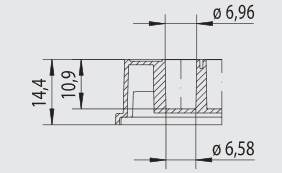
\includegraphics[width=0.5\textwidth]{AfmetingenMicrowell.png}
	\caption{Afmetingen \textit{microwell}}
	\label{fig: afmetingenMicrowellplaat}
	
\end{figure} 


\chapter{Ontwerpen} 
\section{Mogelijke \textit{concepts}}
\subsection{Concept 1}
Een eerste concept is gebaseerd op het principe van een handmatige \textit{dispenser} die ter beschikking werd gesteld. In Figuur \ref{fig: schets concept 1} staat een schets van het \textit{concept}. De \textit{wells} worden in dit concept in een keer gevuld door 96 cilinders. De cilinders zijn vastgemaakt aan een plaat in 12 rijen van 8. De afstand tussen de middelpunten van 2 cilinders is telkens 9 mm. De cilinders zelf bewegen niet. In elke cilinder zit een zuiger die op en neer kan bewegen. De koppen van de cilinders zijn vastgemaakt op een plaat die op en neer kan bewegen (zie Figuur \ref{fig: foto concept 1 zuiger}) m.b.v. een motor die boven het geheel van de twee platen is bevestigd. Het geheel van de platen met de zuigers en cilinders kan op en neer bewegen om de vloeistof in de cilinders op te zuigen. De \textit{microwell}-plaat is bevestigd aan een aandrijfriem met een motor zodat de plaat naar links en rechts kan bewegen. Dit laat het mechanisme toe om telkens de cilinders opnieuw te vullen en een gevulde \textit{microwell}-plaat te vervangen door een lege.  

\begin{figure}[h]
	\centering
	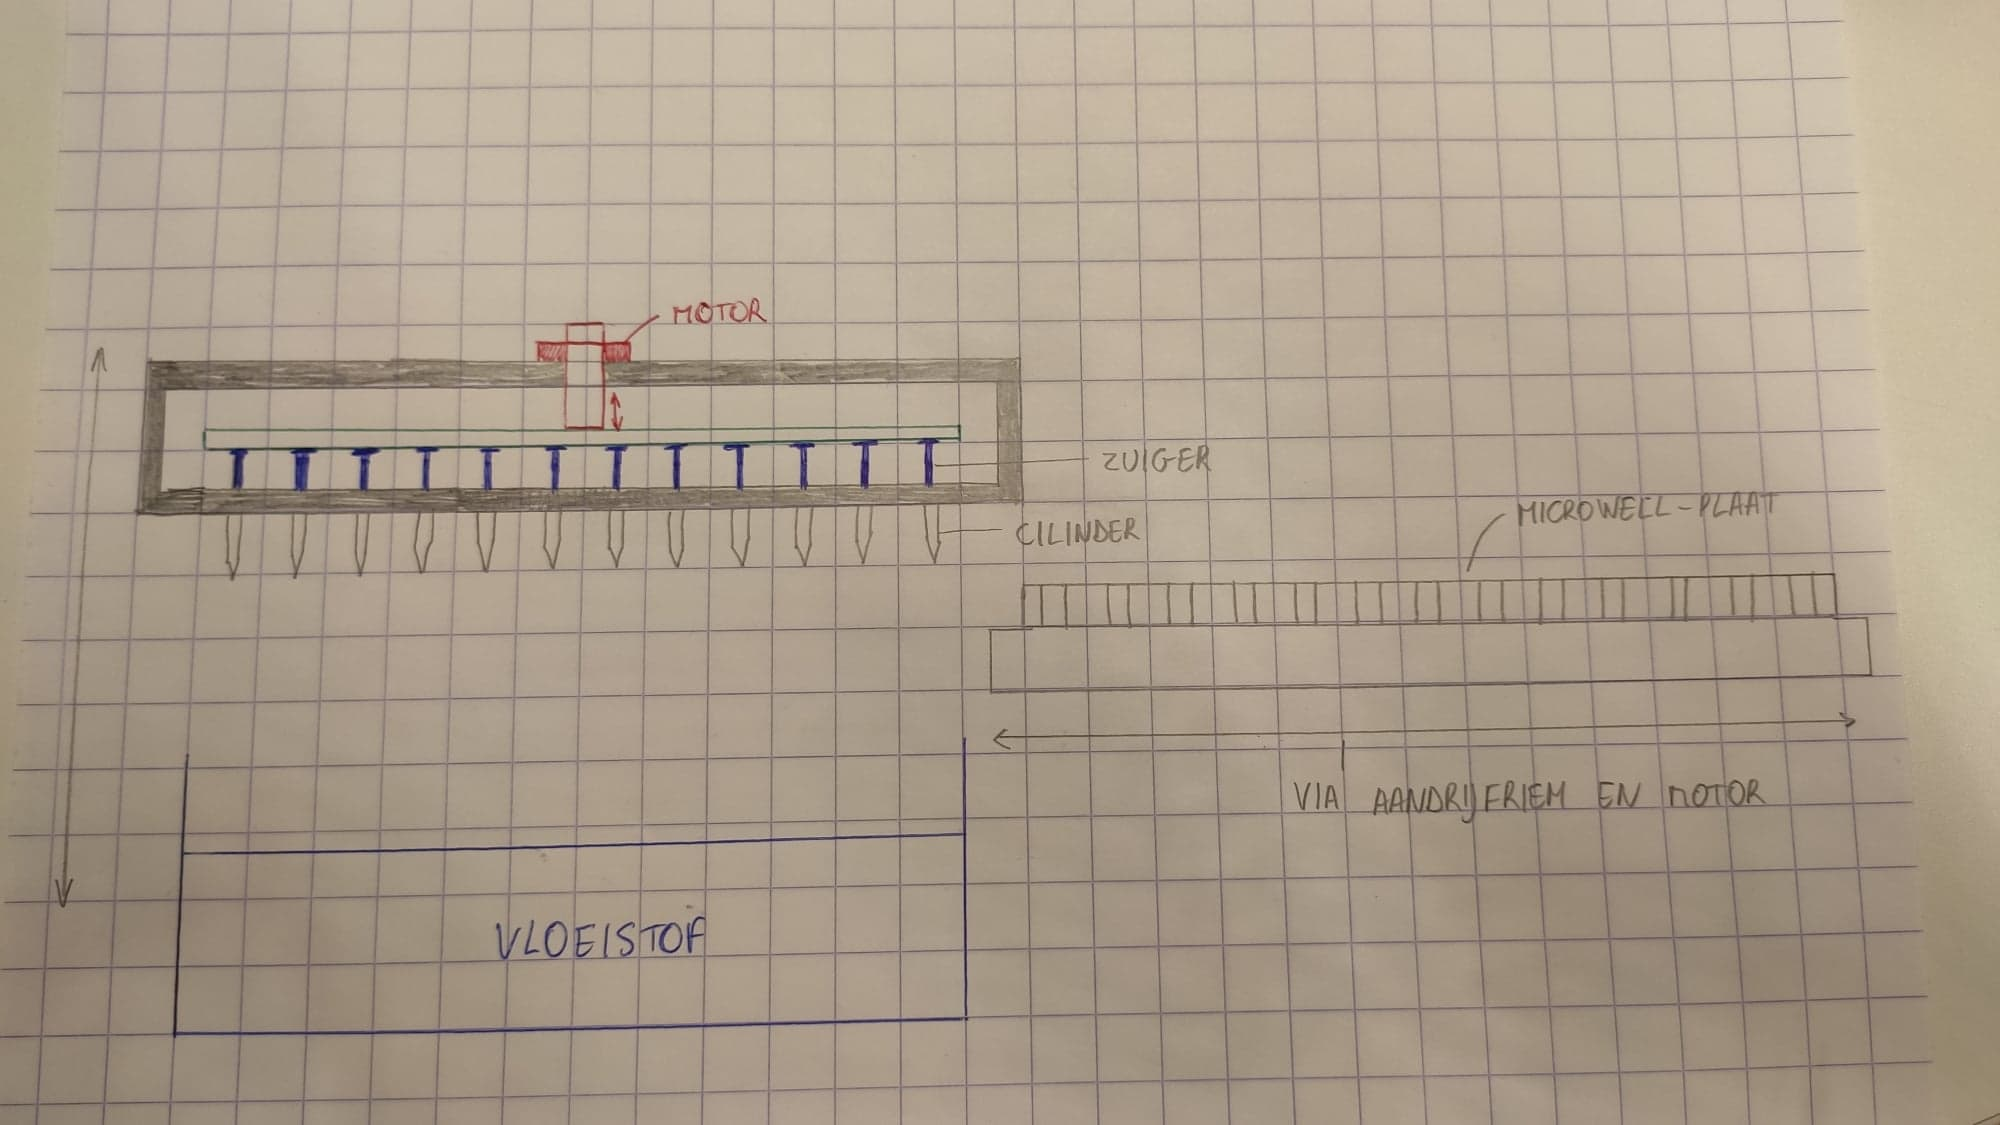
\includegraphics[width=0.8\textwidth]{fotoConcept1.jpg}
	\caption{Schets \textit{concept} 1}
	\label{fig: schets concept 1}
	
\end{figure} 

\begin{figure}
	\centering
	\begin{subfigure}{.5\textwidth}
		\centering
		\includegraphics[width=0.7\linewidth,angle=270]{fotoConcept1Zuiger(1).jpg}
		\caption{Plaat aan de koppen van de zuigers omhoog}
	\end{subfigure}%
	\begin{subfigure}{.5\textwidth}
		\centering
		\includegraphics[width=0.7\linewidth,angle=270]{fotoConcept1Zuiger(2).jpg}
		\caption{Plaat aan de koppen van de zuigers omlaag}
	\end{subfigure}
	\label{fig: foto concept 1 zuiger}
\end{figure}

\subsection{Concept 2}
Het tweede concept is qua mechanisme om de \textit{wells} te vullen gelijkaardig, alleen worden hier minder cilinders en zuigers gebruikt. In Figuur \ref{fig: schets concept 2} staat een schets van het \textit{concept}. Er worden acht cilinders naast elkaar vastgemaakt aan een plaat, met opnieuw een afstand van 9 mm tussen de middelpunten van twee aanliggende cilinders. De zuigers die in de cilinders zitten, worden op analoge manier bevestigd als in \textit{concept} 1. In plaats van de \textit{wells} in de plaat in een keer te vullen, gebeurt dit nu in twaalf stappen. Telkens wanneer een rij van acht \textit{wells} gevuld is, schuift de \textit{microwell}-plaat naar rechts, tot deze zich niet meer onder de zuigers bevindt, en beweegt het geheel met de zuigers en cilinders naar onder en weer naar boven om de cilinders opnieuw te vullen met vloeistof. Vervolgens schuift de \textit{microwell}-plaat opnieuw naar links onder de cilinders en wordt de volgende rij van 8 \textit{microwells} gevuld.

\begin{figure}[h]
	\centering
	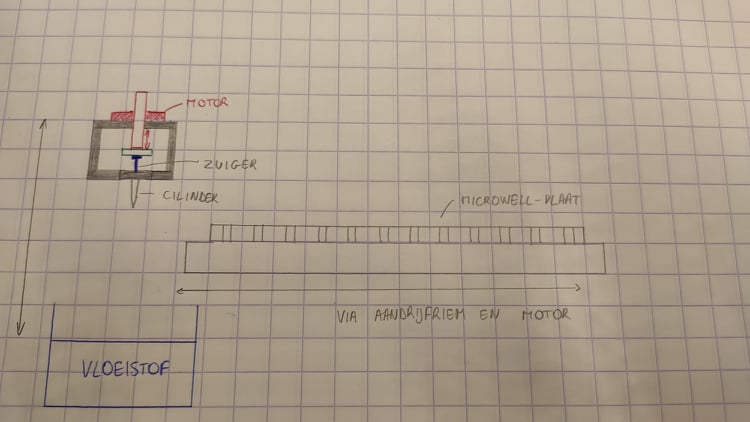
\includegraphics[width=0.8\textwidth]{fotoConcept2.jpg}
	\caption{Schets \textit{concept} 2}
	\label{fig: schets concept 2}
	
\end{figure} 

\subsection{Concept 3}
Het derde \textit{concept} is compleet verschillend van de eerste twee. In dit \textit{concept} (zie Figuren \ref{fig: CAD-model globaal} en \ref{fig: CAD-model ingezoomd}) wordt gewerkt met een pomp die de vloeistof uit het recipiënt oppompt en via een buizennetwerk verdeelt over acht pipetpunten waarvan de middelpunten zich opnieuw op een afstand van 9 mm van elkaar bevinden. De afstand die de vloeistof aflegt van de pomp tot aan de uitgang van de pipetpunt is voor elk van de acht kanalen gelijk, wat belangrijk is om in elke \textit{well} even veel vloeistof te hebben. De \textit{microwell}-plaat wordt vastgemaakt aan een aandrijfriem en motor en kan op die manier verplaatst worden. Telkens wanneer een rij van acht \textit{wells} gevuld is, stopt de pomp en verschuift de \textit{microwell}-plaat 9 mm naar links. Daarna vult de pomp opnieuw acht \textit{wells}. Dit proces wordt herhaald tot de twaalf rijen van acht \textit{wells} gevuld zijn. 

\begin{figure}[h]
	\centering
	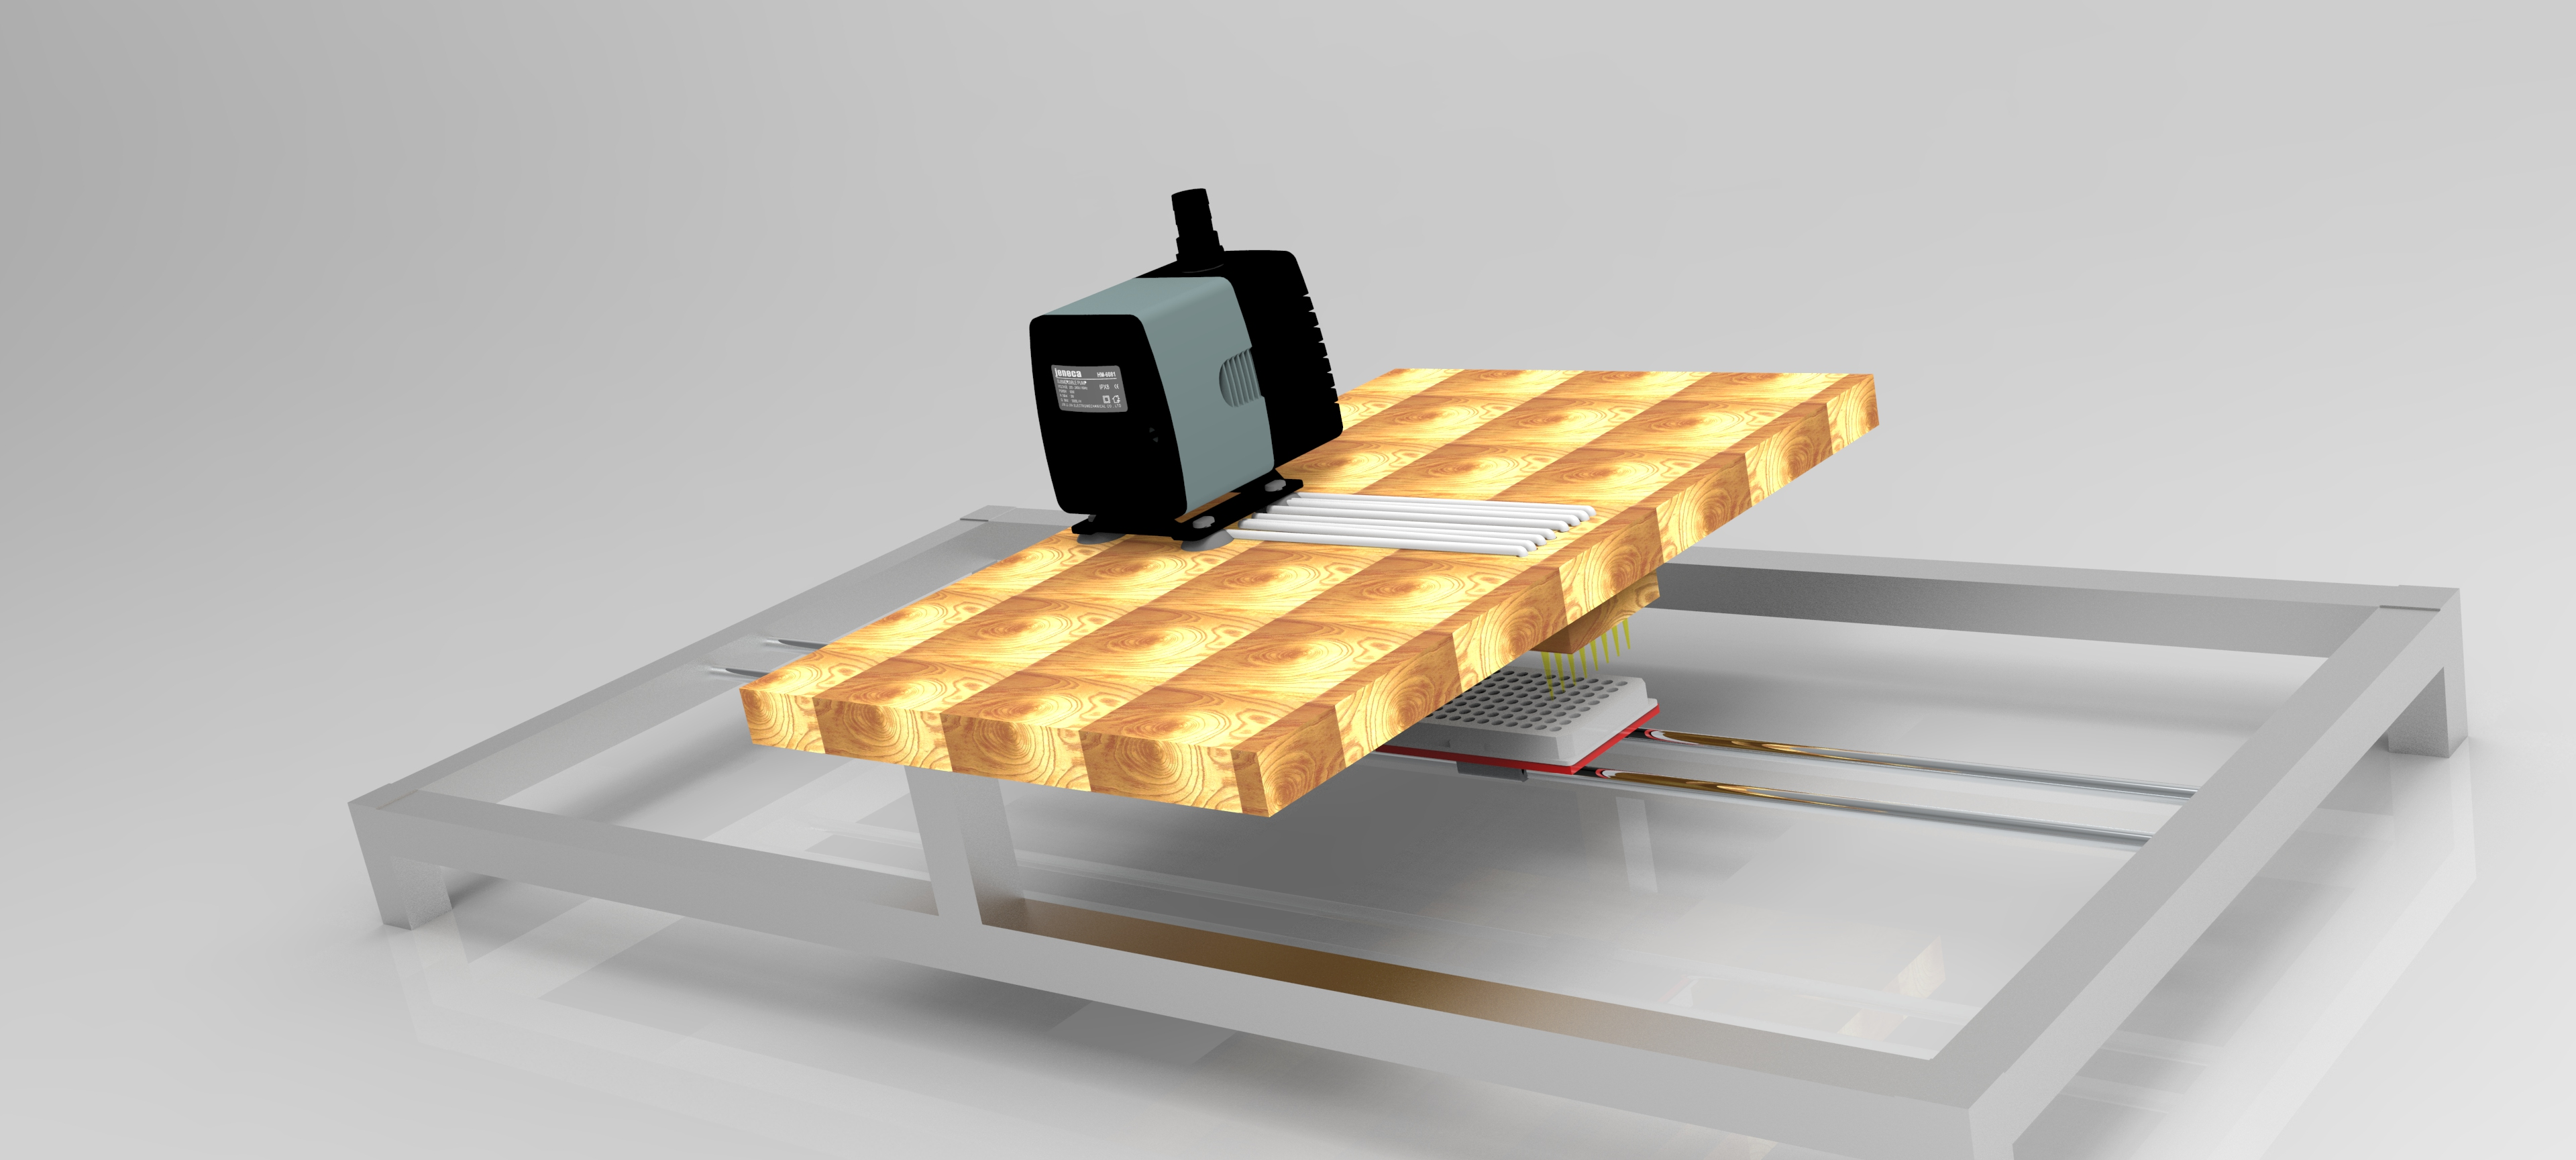
\includegraphics[width=0.8\textwidth]{micdis1.jpg}
	\caption{CAD-model \textit{concept} 3}
	\label{fig: CAD-model globaal}
	
\end{figure} 

\begin{figure}[h]
	\centering
	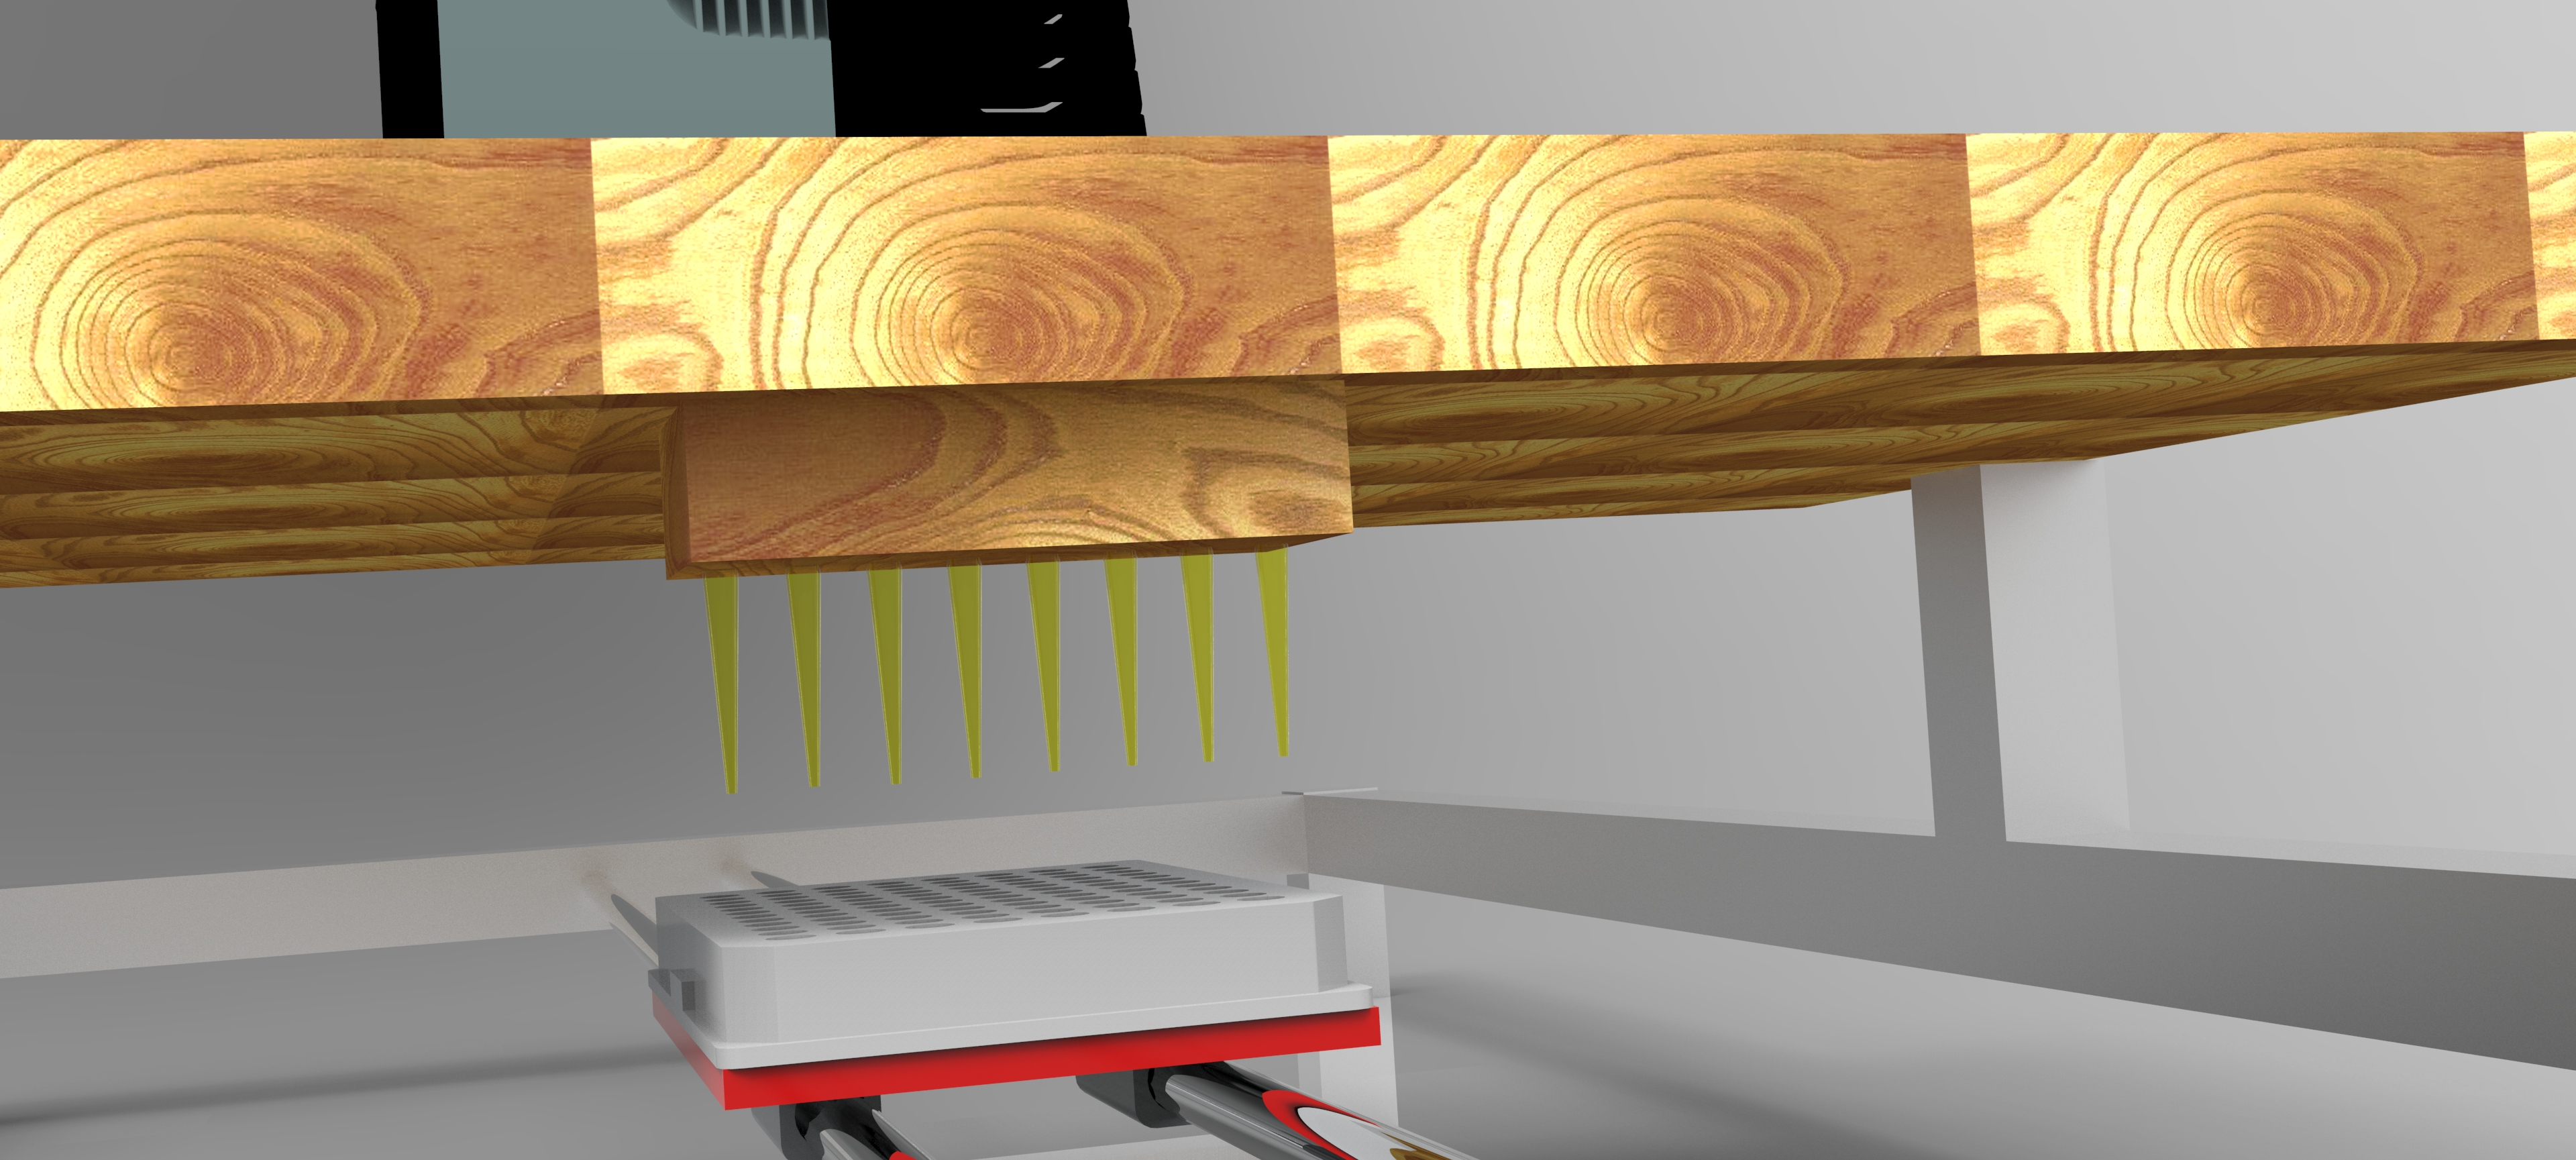
\includegraphics[width=0.8\textwidth]{micdis2.jpg}
	\caption{CAD-model \textit{concept} 3}
	\label{fig: CAD-model ingezoomd}
	
\end{figure} 

\section{Selectie concept}
In deze sectie worden per ontwerp de voordelen opgesomd en wordt de uiteindelijke keuze van een van de drie \textit{concepts} toegelicht.

\subsection{Voordelen}

\paragraph{Concept 1}
\begin{itemize}
	\item Snelste optie, want alle 96 \textit{wells} in één keer gevuld
	\item Uiterst precies, want er wordt gewerkt met vooraf geijkte cilinders zodat elke 	\textit{well} exact even veel vloeistof krijgt
\end{itemize}

\paragraph{Concept 2}
\begin{itemize}
	\item Goedkoper dan \textit{concept} 1
	\item Uiterst precies, want er wordt gewerkt met vooraf geijkte cilinders zodat elke 	\textit{well} exact even veel vloeistof krijgt
\end{itemize}

\paragraph{Concept 3}
\begin{itemize}
	\item Sneller dan \textit{concept 2}, want geen verticale bewegingen nodig
	\item Goedkoopste optie
	\item Eenvoudiger te maken dan \textit{concept} 1 en 2, want geen bewegingen in twee dimensies nodig
\end{itemize}

\subsection{Selectie uiteindelijk ontwerp}
Uiteindelijk werd gekozen voor \textit{Concept} 3. De doorslaggevende factor was hierbij de kostprijs. In het eerste en tweede \textit{concept} kosten de gebruikte zuigers en cilinders per stuk evenveel als het voorziene budget voor de gehele machine. Aangezien deze niet nodig waren voor het derde concept, is dit veruit het goedkoopste effect. Doordat enkel de plaat horizontaal moet kunnen bewegen, hebben we maar een riem en een \textit{steppermotor} voor dit ontwerp. Bij de eerste twee ontwerpen moet er ook verticale beweging zijn voor de zuigers. Hiervoor zijn een tweede riem en \textit{steppermotor} nodig, wat het productieproces ingewikkelder en duurder maakt. De snelheid van concept drie is afhankelijk van hoe krachtig de pomp is. Wanneer deze voldoende snel de substantie kan opzuigen en spuiten, zal dit concept zeker sneller zijn dan concept twee en amper trager dan concept een. Indien de pomp nauwkeurig genoeg is en er gewerkt wordt met precies even lange en dikke buizen, kan men ook exact de gevraagde hoeveelheid subsantie in de \texit{wells} spuiten. 





\chapter*{Appendices}
\section*{Financieel verslag}

In Tabel \ref{tab:financieelVerslag} staan de gemaakte aankopen vermeld. VOOR DE VERZENDING WERD NOG EEN EXTRA BEDRAG VAN    BETAALD.


\begin{table}[]
	\sffamily
	\label{tab:financieelVerslag}
	\caption{Aankopen}
	\begin{tabular}{@{}lllll@{}}
		\toprule
		  Item & Product & Prijs/stuk (\euro) & Aantal & Totaal (\euro)   \\ \midrule
		1 & Staaf voor X- of Y-as glad 10 mm x 100 cm & 4.75 & 2 & 9.50 \\
		2 & SCS10UU lineaire kogellager  & 5.50 & 2 & 11.00 \\
		3 & GT2 timing belt 6 mm (per meter)  & 4.50 & 2 & 9.00 \\
		4 & GT2 Pulley hoge resolutie | 6 mm riem | 20 tanden | 5 mm as & 6.00 & 1 & 6.00 \\
		5 & Spanrol | gladde pulley hoge resolutie | 6 mm riem | 5 mm as & 5.50 & 1 & 5.50 \\
		6 & SHF10 as-bevestiging (2 stuks) & 9.50 & 2 & 19.00 \\
		7 & Aluminium profiel 2020 extrusion lengte 1 m (123-3D huismerk)  & 9.50 & 3 & 28.50 \\
		8 & Aluminium hoekverbinding 2020 inclusief bevestigingsmateriaal (123-3D huismerk) & 2.75 & 4 & 11.00 \\
		9 & Hulpstukje 4 mm Luchtslang PE T-stuk 4 x 4 x 4 mm & 0.20 & 15 & 3.00 \\
		\bottomrule
	\end{tabular}

	
\end{table}

\clearpage

\section*{Verantwoordelijkheden taakverdeling}

De volledige opdracht werd verdeeld in volgende delen (met bijhorende verantwoordelijken):
\begin{itemize}
	\item \textsc{Teamleider:} Seppe Vilain
	\item \textsc{Notulist}: Maxime Dujardin
	\item \textsc{Opstellen CAD-model}: Korneel Verkens
	\item \textsc{Mechanisme om platform met \textit{microwell}-platen te verplaatsen:} Matthias Derez, Seppe Vilain
	\item \textsc{Pompsysteem:} Maxime Dujardin, Korneel Verkens
	\item \textsc{Verslag \& presentatie:} Matthias Derez, Maxime Dujardin, Korneel Verkens, Seppe Vilain
	
\end{itemize}

\clearpage

\section*{Vakintegratie}
Om dit project tot een goed einde te kunnen brengen werden een aantal vakken uit semesters 1 t.e.m. 3 gebruikt:

\paragraph{Algemene Natuurkunde: Mechanica}

In het vak 'Mechanica' werden de basisbeginselen i.v.m. druk en stroming in dunne buizen bijgebracht. Deze kennis werd gebruikt bij het ontwerpen van het buizensysteem om de vloeistof te verdelen naar de acht \textit{microwells}.

\paragraph{Beginselen van Programmeren}

De gebruikte programmeertaal voor de programma's die de machine gebruikt, is Python. In het vak 'Beginselen van Programmeren' werd deze taal geleerd. 

\paragraph{Probleemoplossen \& Ontwerpen, deel 2}

Het CAD-model werd gemaakt met het programma 'Solid Edge'. In P\&O 2 werd aangeleerd hoe hiermee te werken. Verder werd hier ook getoond hoe een \textit{Raspberry Pi microcontroller} kan bestuurd worden vanaf een computer. 

\paragraph{Algemene Natuurkunde: Elektromagnetisme en Informatieoverdracht en -verwerking \& elektrische netwerken}

Deze vakken behandelen o.a. het maken en oplossen van elektrische circuits en overdracht van informatie, wat van pas kwam bij het maken van de connecties tussen de vacuümpomp, de \textit{stepper}motor, de \textit{Raspberry Pi microcontroller}, \textit{mosfet} ... en de computer.

\section*{Vergaderverslagen}
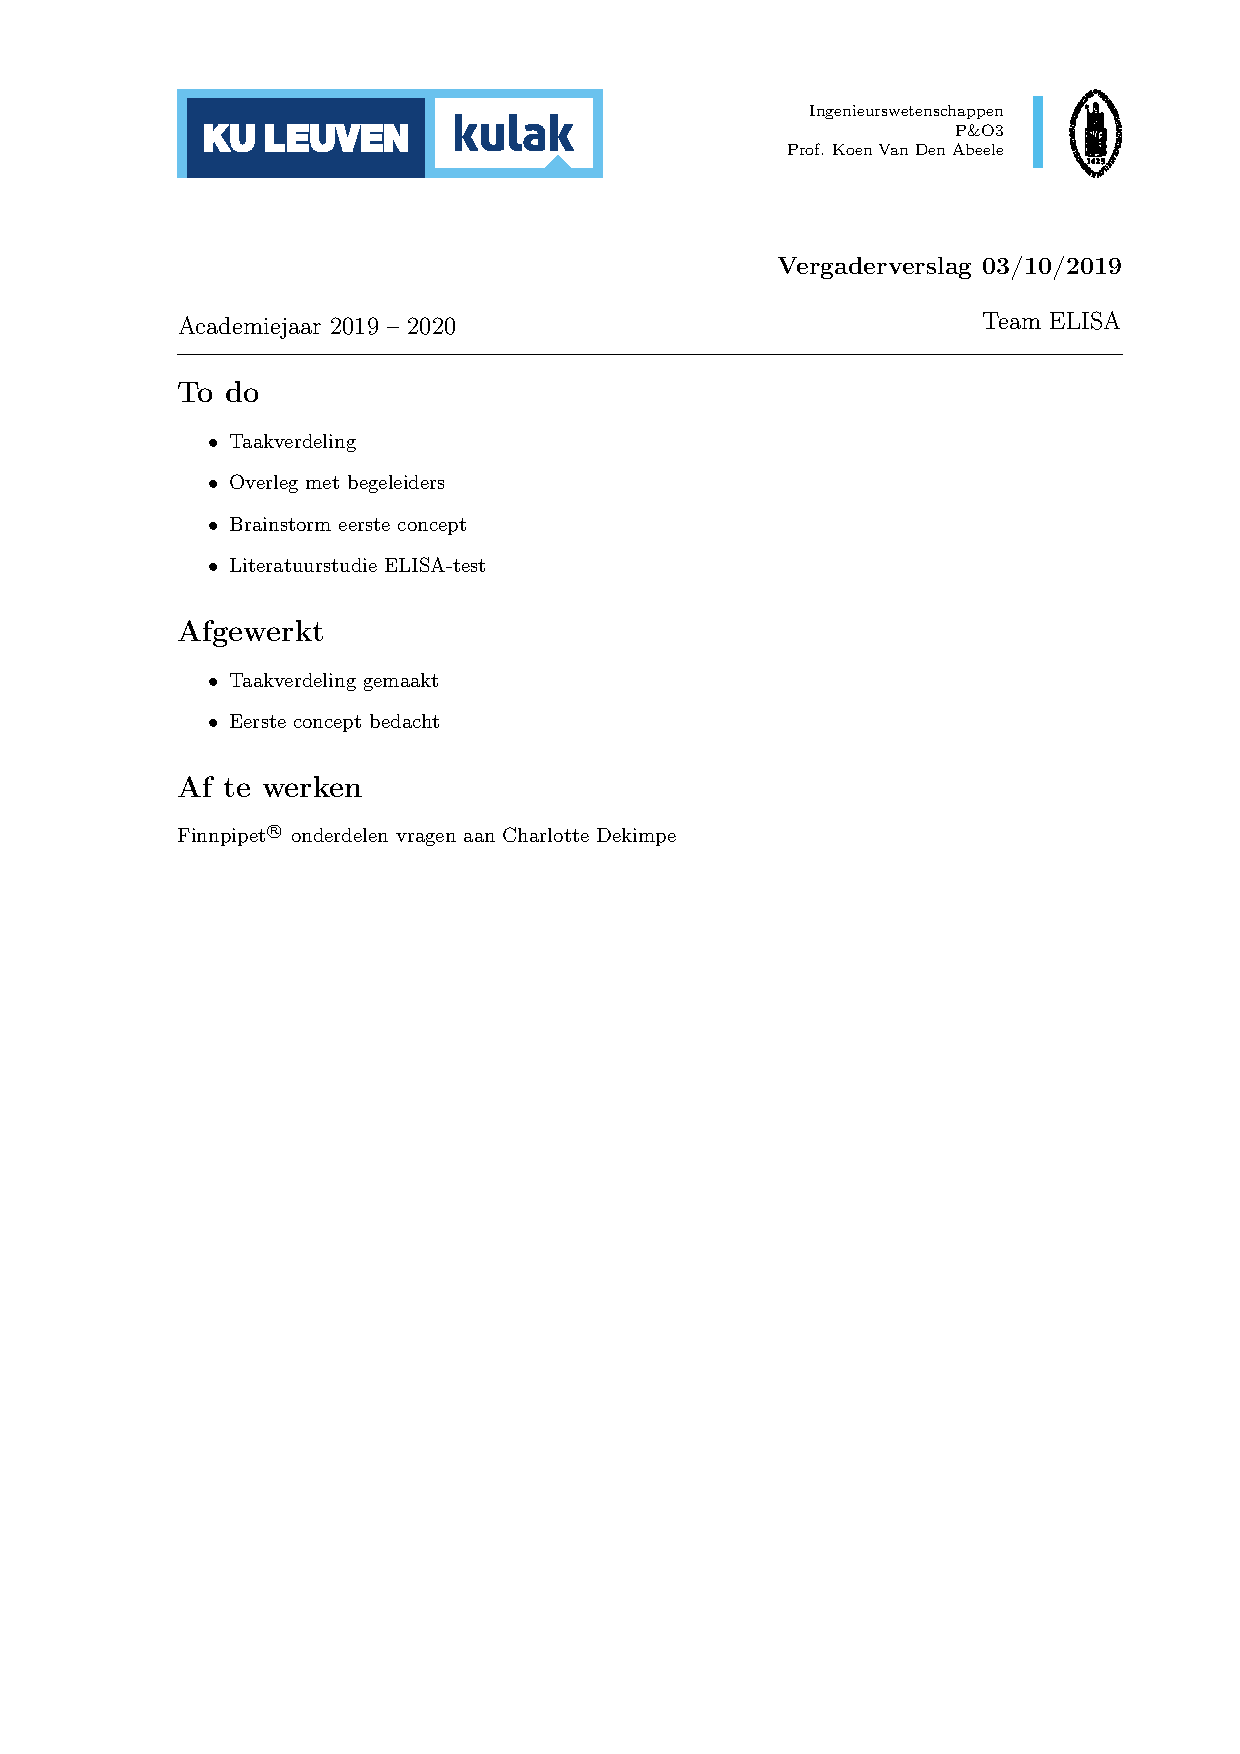
\includepdf{vergaderverslag3oktober.pdf}
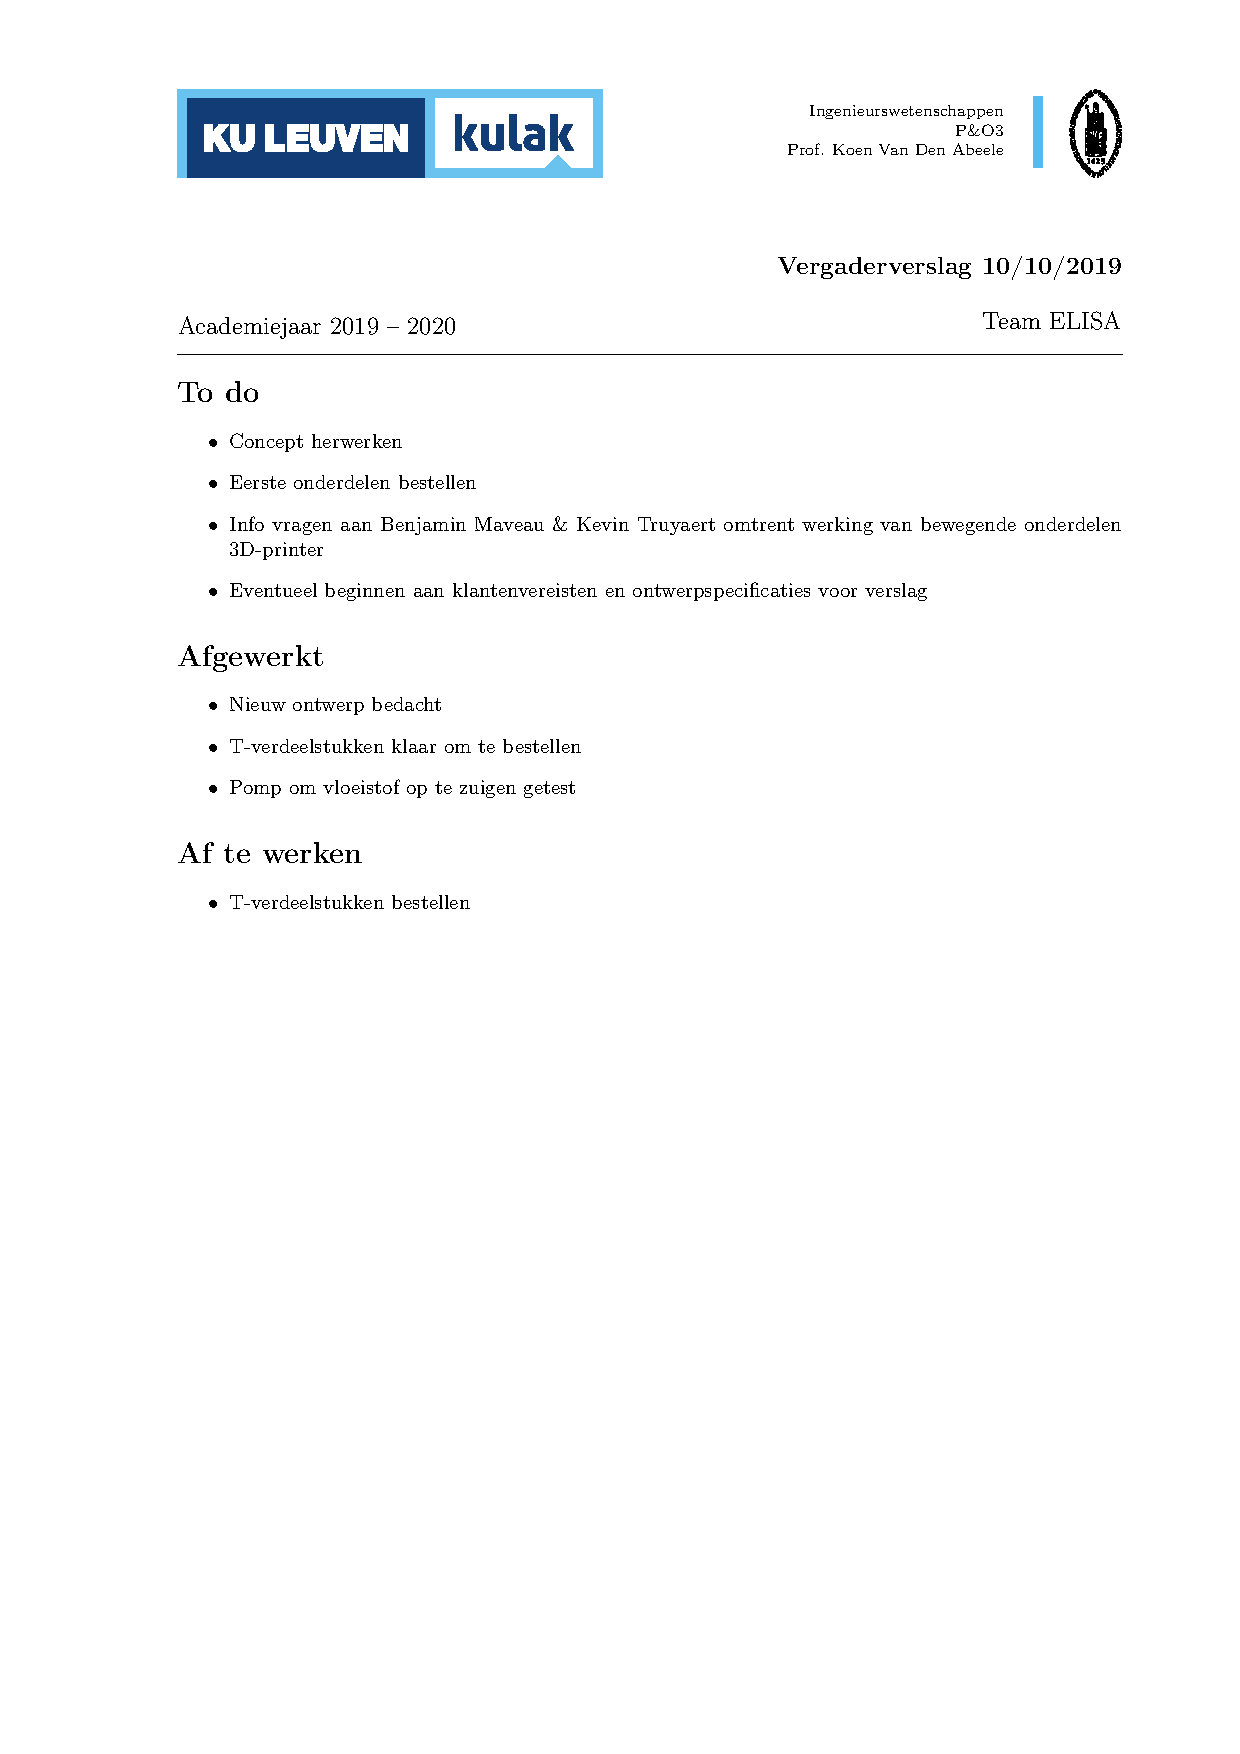
\includepdf{vergaderverslag10oktober.pdf}
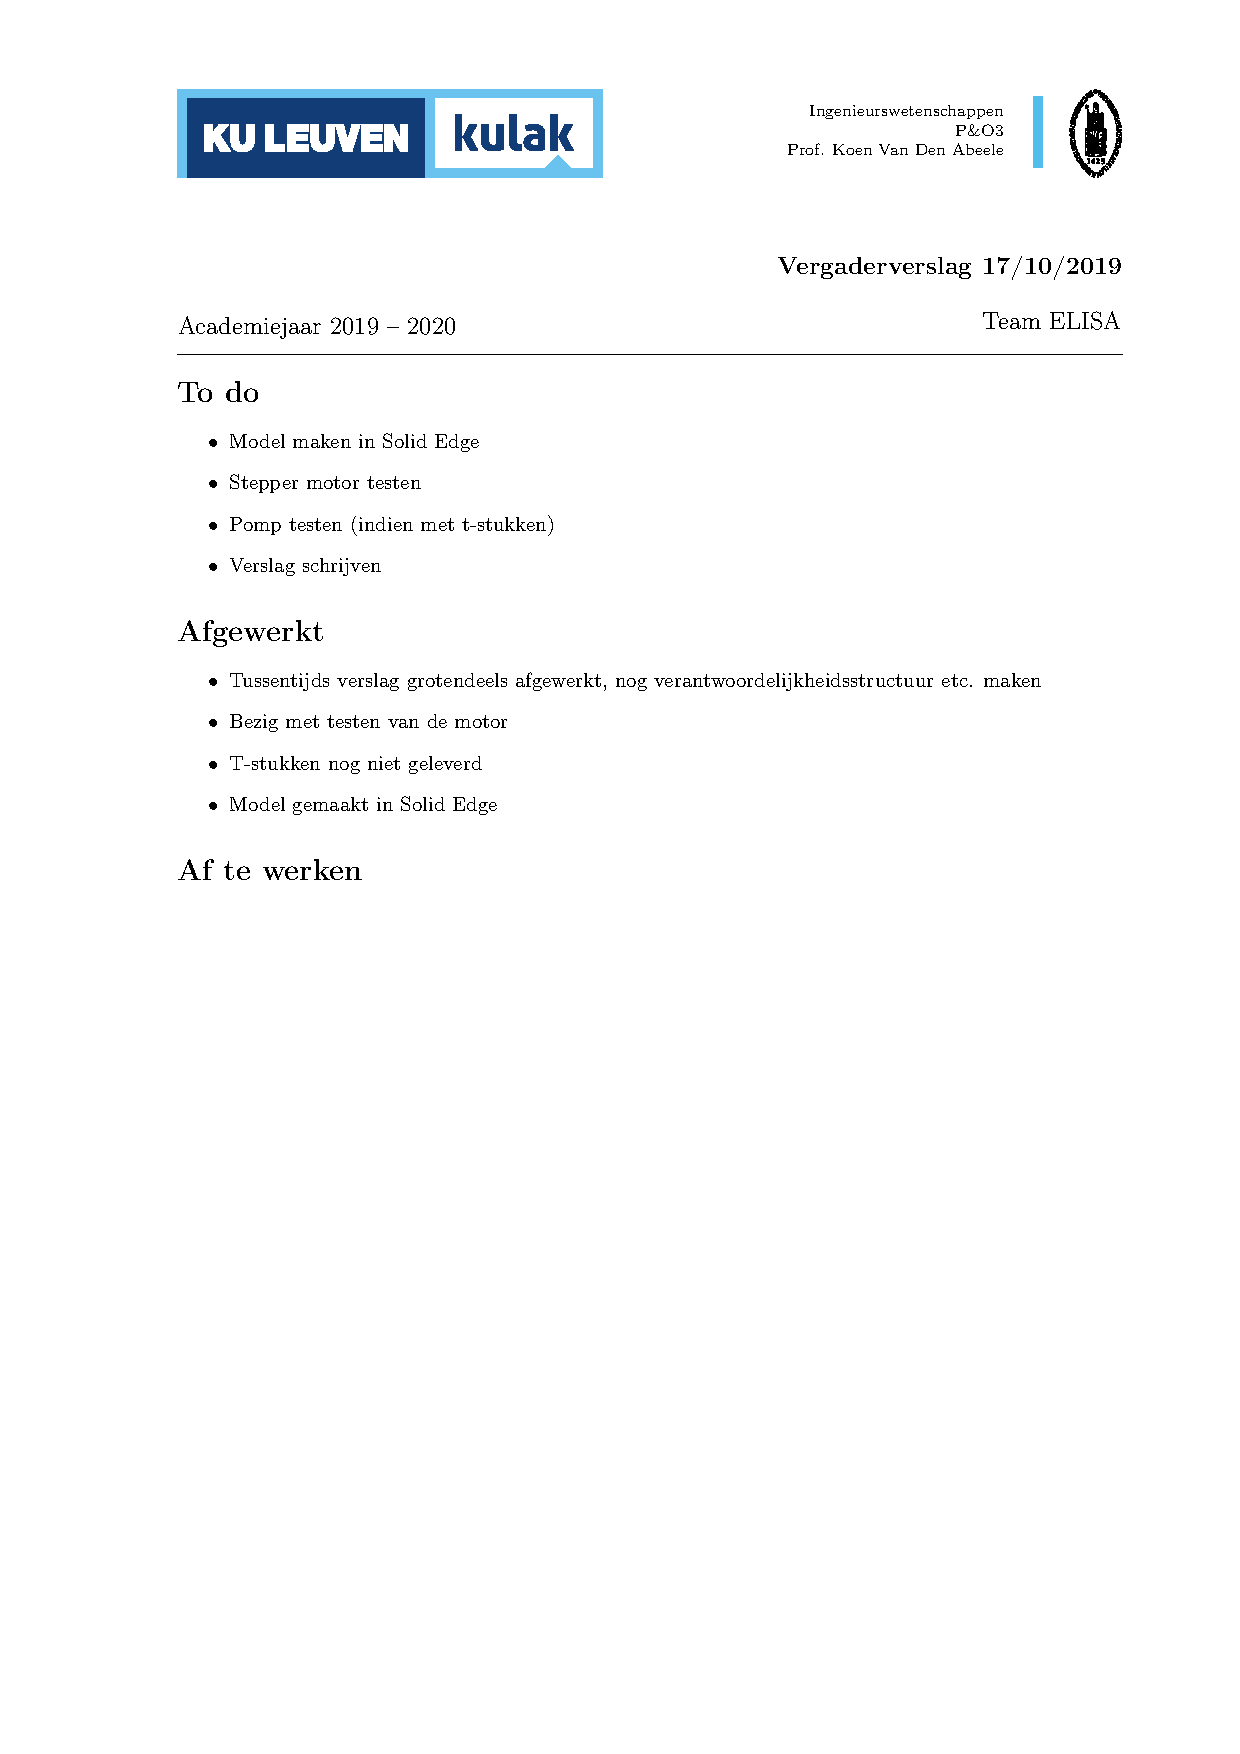
\includepdf{vergaderverslag17oktober.pdf}
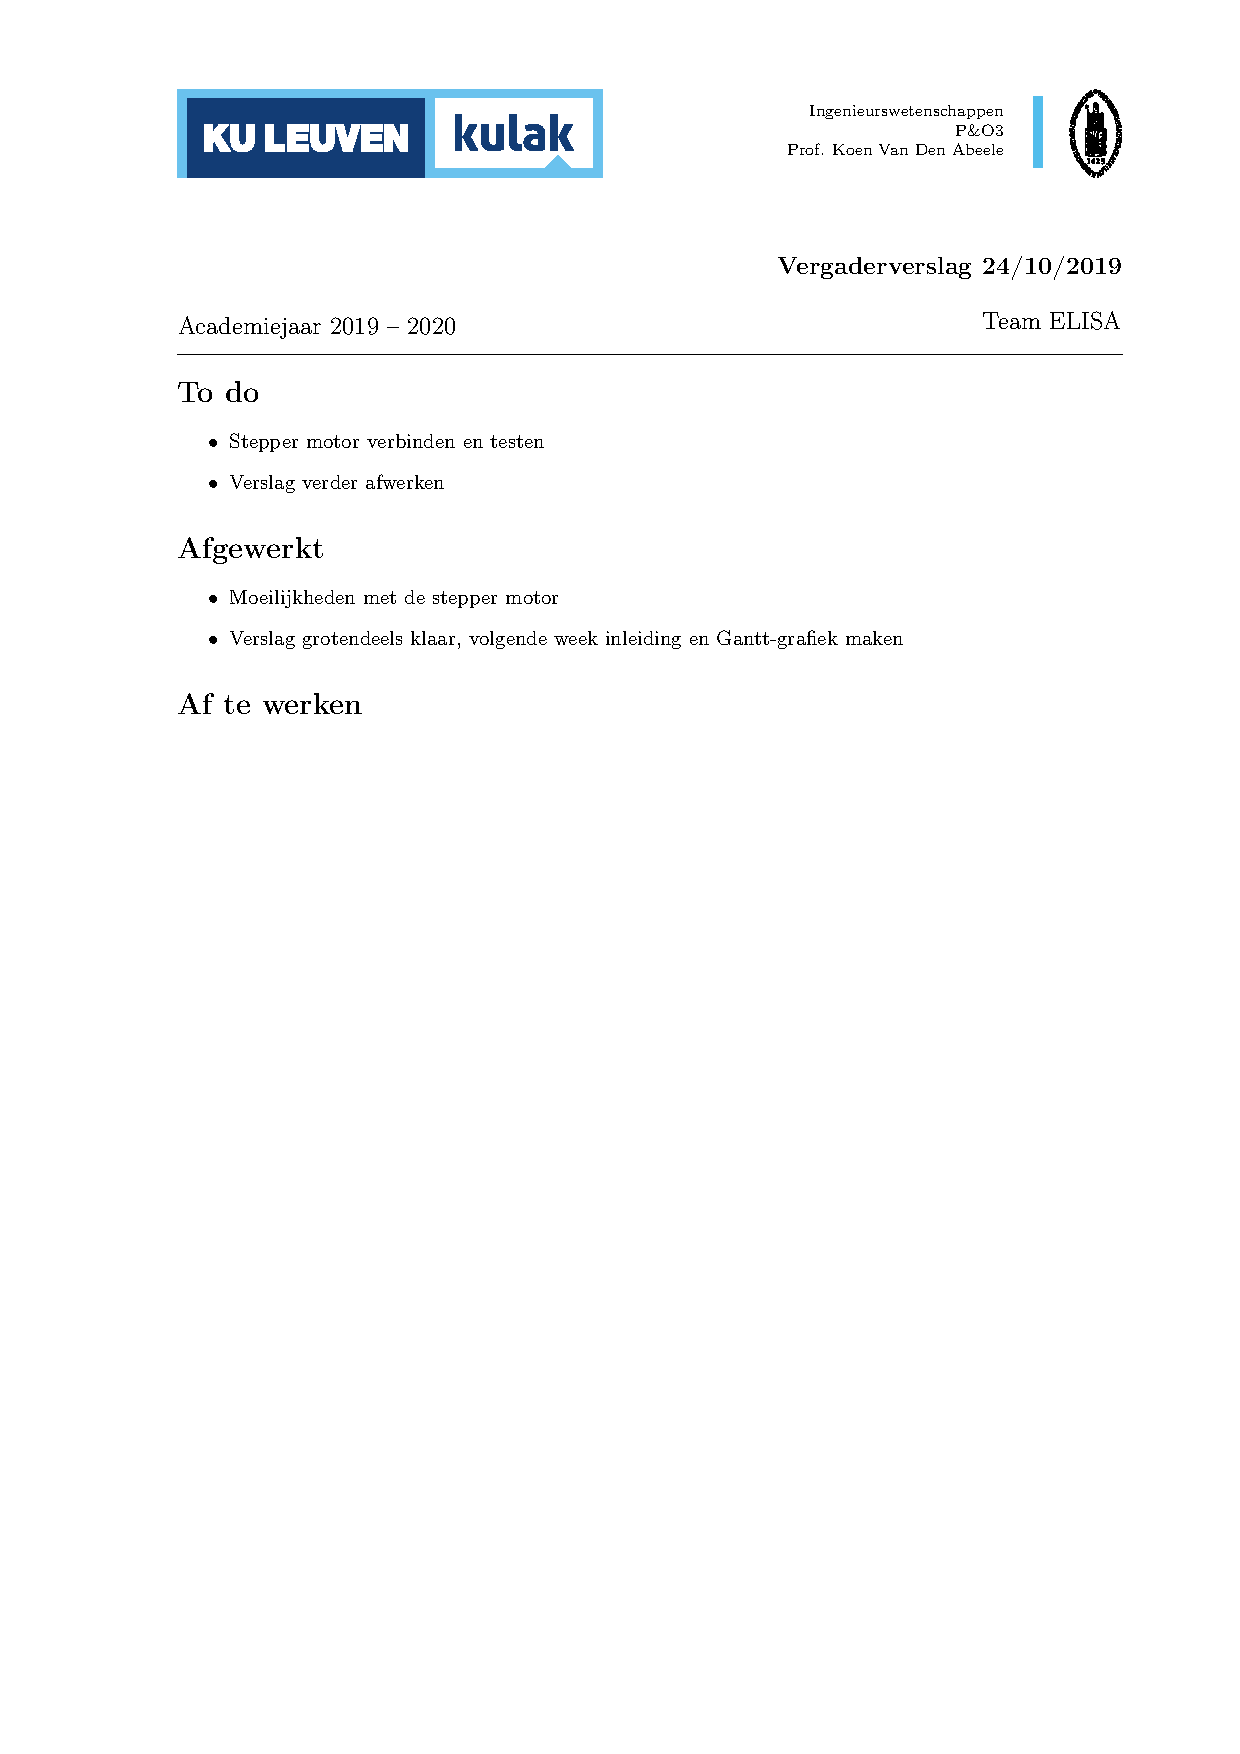
\includepdf{vergaderverslag24oktober.pdf}
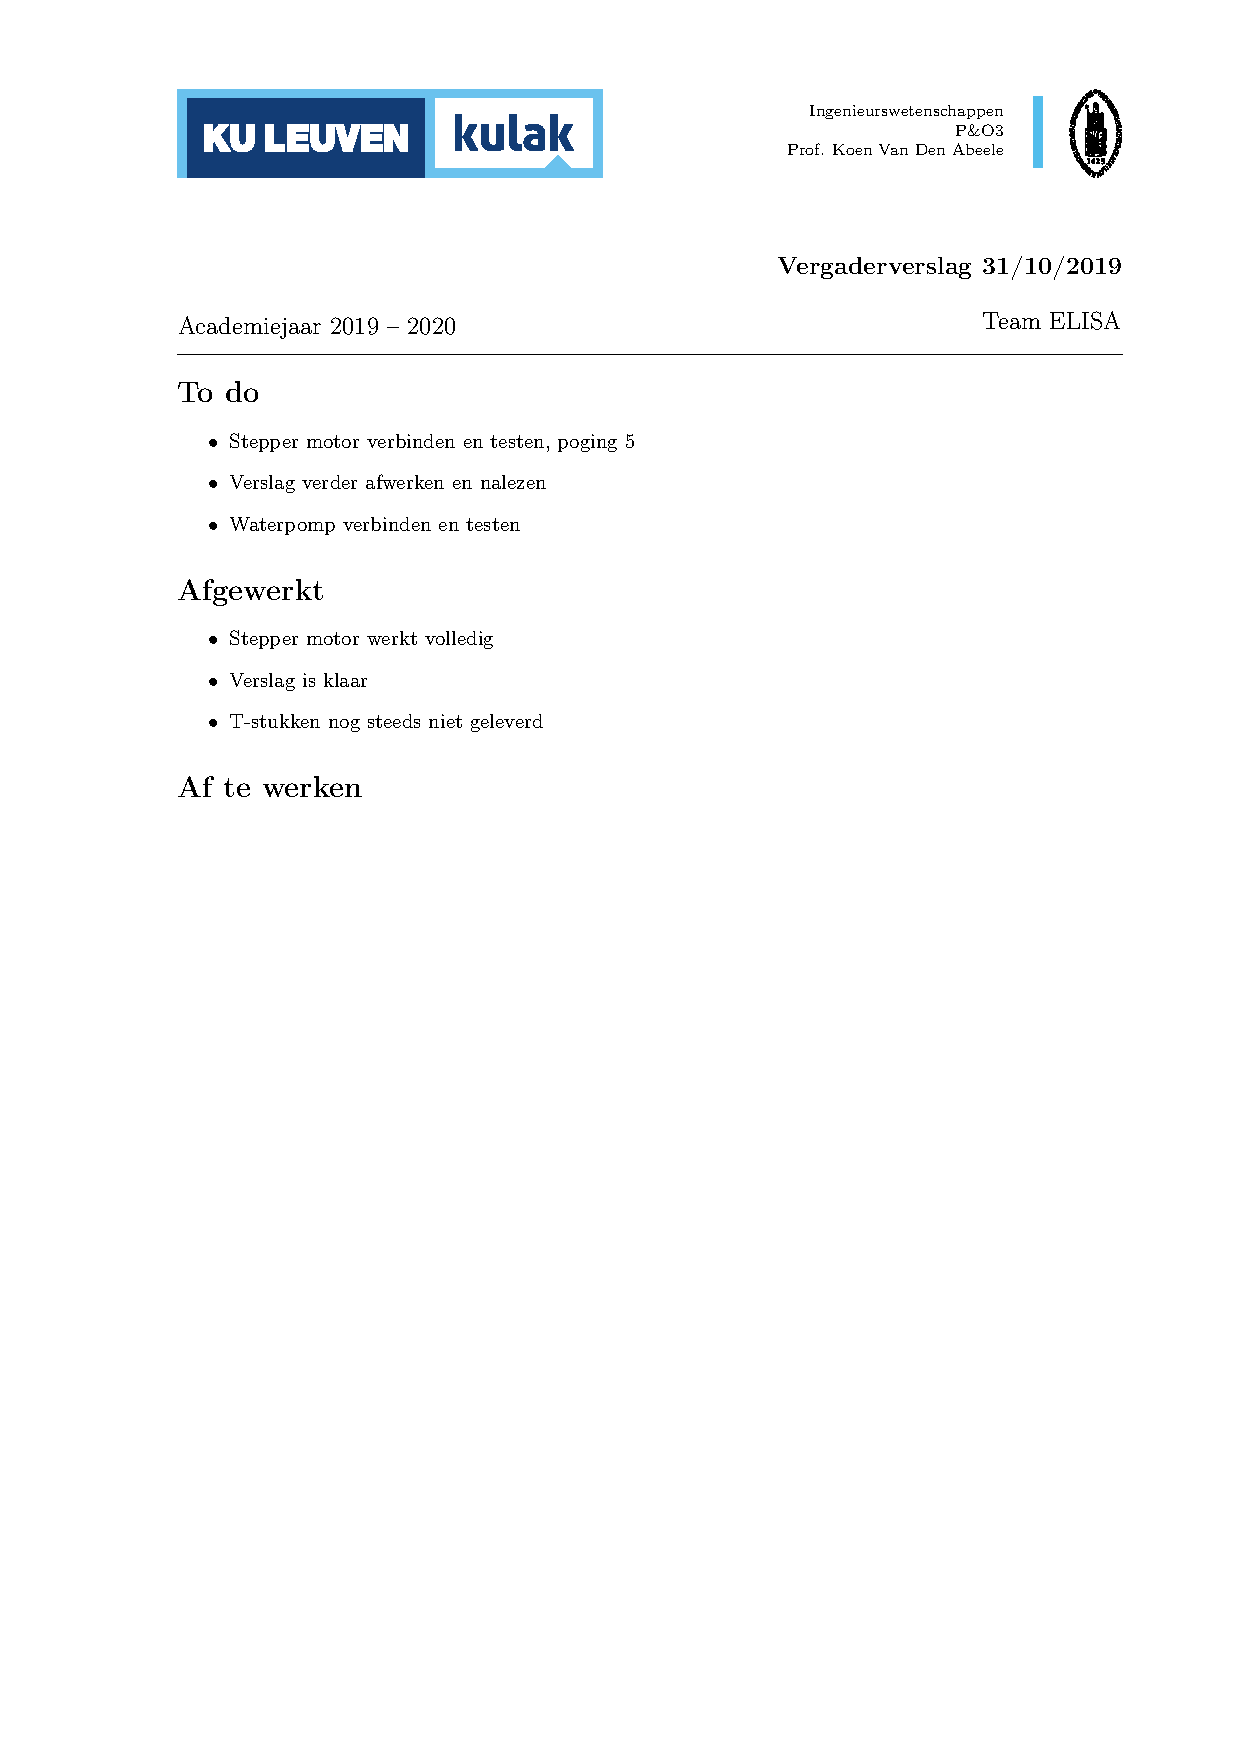
\includepdf{vergaderverslag31oktober.pdf}

 




\end{document}
